\section{Result 1: a threshold on peak contrast}
\label{sec:result-1}

$\cH=\{h_\theta\}$ with $h_\theta(x)=+1$ iff $x>\theta$, on the scalar peak contrast $x$ (the
maximum of the difference image over the candidate). The learner is exact ERM: sort the $n$
training values, sweep the $n+1$ cuts with cumulative sums, and put $\hat\theta$ at the midpoint
of the chosen gap. $L(h)=\P_Q(h(x)\ne y)$ and $\hat L_S(h)$ is the training error.

$\cH$ has VC dimension $d=1$: one point is shattered ($\theta$ below or above it), but for
$x_1<x_2$ the labelling $(+1,-1)$ would need $x_1>\theta\ge x_2$. By the Sauer--Shelah lemma the
growth function, the number of labellings $\cH$ induces on $m\ge d$ points, satisfies
$\Pi_\cH(m)\le(em/d)^d$; for thresholds, $\Pi_\cH(2n)\le2en$.

\begin{theorem}[Result 1]
\label{thm:1}
Let $\hat h$ be any ERM hypothesis on $n$ i.i.d.\ examples from $Q$, and $h^\star\in\argmin_\cH L$.
\begin{enumerate}[label=(\roman*)]
  \item (Realizable.) If $L(h^\star)=0$ and $0<\delta\le1/2$, then with probability at least
  $1-\delta$
  \[ L(\hat h)\le\frac{2}{n\ln 2}\Bigl(\ln(2en)+\ln\frac2\delta\Bigr). \]
  \item (Agnostic.) With probability at least $1-\delta$
  \[ L(\hat h)-L(h^\star)\le\sqrt{\frac{32\bigl(\ln(2en)+\ln(4/\delta)\bigr)}{n}}. \]
\end{enumerate}
\end{theorem}

Both parts compare the training sample $S$ with an independent ghost sample $S'$ of size $n$.

\begin{lemma}[Uniform convergence]
\label{lem:uc}
For any class $\cH$ of binary classifiers and $n\epsilon^2\ge2$,
\[ \P\Bigl(\sup_{h\in\cH}\abs{L(h)-\hat L_S(h)}>\epsilon\Bigr)\le4\,\Pi_\cH(2n)\,e^{-n\epsilon^2/8}. \]
\end{lemma}
\begin{proof}
The argument goes back to \citet{vapnik1971uniform}; see also \citet{shalevshwartz2014understanding}.
\emph{Symmetrization.} On the event, pick (as a function of $S$) an $h$ with
$\abs{L(h)-\hat L_S(h)}>\epsilon$. Given $S$, $\hat L_{S'}(h)$ is a mean of $n$ independent
indicators with mean $L(h)$ and variance at most $1/(4n)$, so by Chebyshev
$\P(\abs{\hat L_{S'}(h)-L(h)}\ge\epsilon/2)\le1/(n\epsilon^2)\le1/2$. With probability at least
$1/2$ the two deviations therefore leave $\abs{\hat L_S(h)-\hat L_{S'}(h)}>\epsilon/2$, and
$\P(\sup_h\abs{L-\hat L_S}>\epsilon)\le2\,\P(\sup_h\abs{\hat L_S-\hat L_{S'}}>\epsilon/2)$.
\emph{Swaps.} All $2n$ points are i.i.d., so swapping the $i$-th points of $S$ and $S'$ does not
change the joint law of $(S,S')$, and after conditioning on the $2n$ points a hypothesis matters only
through its labelling of them. Let $\sigma_i=\pm1$ be independent fair signs that swap pair $i$ when $-1$. For a
fixed labelling with losses $a_i,b_i\in\{0,1\}$ on the $i$-th points of $S,S'$,
$\hat L_S-\hat L_{S'}=\frac1n\sum_i\sigma_i(a_i-b_i)$ is a sum of independent terms, each in an
interval of length at most $2/n$, so Hoeffding's inequality gives
$\P(\abs{\cdot}>\epsilon/2)\le2\exp\bigl(-2(\epsilon/2)^2/(n(2/n)^2)\bigr)=2e^{-n\epsilon^2/8}$.
A union bound over the at most $\Pi_\cH(2n)$ labellings and the factor 2 above give the claim.
\end{proof}

\begin{proof}[Proof of \cref{thm:1}]
(i) Let $\epsilon$ be the right-hand side of (i) and $A=\{\exists h:\hat L_S(h)=0,\ L(h)>\epsilon\}$.
Since $L(h^\star)=0$, $h^\star$ is consistent with $S$ almost surely, so every ERM hypothesis is
consistent and $L(\hat h)>\epsilon$ only on $A$.
\emph{Symmetrization.} On $A$, pick a consistent $h$ with $L(h)>\epsilon$. Given $S$, its number
of mistakes on $S'$ is binomial with mean $nL(h)>n\epsilon$ and variance below $nL(h)$, so by
Chebyshev it is below $nL(h)/2$ with probability at most $4/(nL(h))<4/(n\epsilon)\le1/2$, using
$n\epsilon=\frac{2}{\ln2}(\ln(2en)+\ln\frac2\delta)\ge\frac{2}{\ln2}(\ln(2e)+\ln4)>8$ for $n\ge1$,
$\delta\le\frac12$. Hence
$\P(A)\le2\,\P(\exists h:\hat L_S(h)=0,\ h\text{ errs on}\ge n\epsilon/2\text{ points of }S')$.
\emph{Swaps.} Fix the $2n$ points and a labelling with $k\ge n\epsilon/2$ mistakes. If some pair
$i$ holds two mistakes, $S$ always contains one. Otherwise the mistakes sit in $k$ different
pairs and all of them land in $S'$ with probability $2^{-k}\le2^{-n\epsilon/2}$.
\emph{Union bound.} $\P(A)\le2\,\Pi_\cH(2n)\,2^{-n\epsilon/2}\le2(2en)\exp\bigl(-\tfrac{n\epsilon\ln2}2\bigr)
=2(2en)\exp\bigl(-\ln(2en)-\ln\tfrac2\delta\bigr)=\delta$.

(ii) $L(\hat h)-L(h^\star)=[L(\hat h)-\hat L_S(\hat h)]+[\hat L_S(\hat h)-\hat L_S(h^\star)]+[\hat L_S(h^\star)-L(h^\star)]$,
and the middle term is $\le0$ for ERM, so the excess is at most $2\sup_h\abs{L(h)-\hat L_S(h)}$.
\Cref{lem:uc} at $\epsilon/2$ with $d=1$ gives $\P(L(\hat h)-L(h^\star)>\epsilon)\le4(2en)e^{-n\epsilon^2/32}$,
which equals $\delta$ at the right-hand side of (ii). The lemma's condition
$n(\epsilon/2)^2=8(\ln(2en)+\ln\frac4\delta)\ge2$ holds.
\end{proof}

\begin{inshort}
\begin{enumerate}[leftmargin=*]
  \item Thresholds have VC dimension 1, so $\Pi(2n)\le2en$.
  \item Realizable: a bad consistent $h$ makes $\ge n\epsilon/2$ mistakes on a ghost sample; random
    swaps put them all there with probability $\le2^{-n\epsilon/2}$; union over $2en$ labellings;
    solve for $\epsilon$: $\tilde O(1/n)$.
  \item Agnostic: excess $\le2\times$ uniform deviation; ghost sample, swaps and Hoeffding give
    $e^{-n\epsilon^2/32}$; union; solve: $\tilde O(1/\sqrt n)$.
  \item Both are worst cases over distributions: some distribution forces each rate, but a given
    one can be learned faster.
\end{enumerate}
\end{inshort}

\paragraph{Measured vs.\ theory (E1).} $\EOneRepeats$ repeats on fresh dies, $n=2^4,\dots,2^{14}$
(nested prefixes). $\hat h$ and $h^\star$ (ERM on the population pool) are evaluated on the same
test pool, so its noise largely cancels in the excess. Slopes are fitted where the mean is at
least $5\times$ the pool noise floor, and their ranges were fixed before running.

\begin{center}
\small
\begin{tabular}{lccc}
\toprule
regime & fitted slope (points) & range fixed in advance & bound above mean at every $n$ \\
\midrule
separable (test error) & $\EOneSepSlope$ ($\EOneSepFitPoints$) & $[-1.15,-0.85]$: \EOneSepSlopePass & \EOneSepBoundPass \\
overlapping (excess error) & $\EOneOvlSlope$ ($\EOneOvlFitPoints$) & $[-1.15,-0.45]$: \EOneOvlSlopePass & \EOneOvlBoundPass \\
\bottomrule
\end{tabular}
\end{center}

Both bounds hold in every run at every $n$, which is the test of the theory; the slopes are
descriptive. The overlapping excess falls faster than the worst case $n^{-1/2}$: the nuisance
density ends sharply at $\theta^\star$, where $P(\text{defect}\mid\text{contrast})$ jumps from
$\OvlCondBelow$ to $\OvlCondAbove$. Such a near-jump at the optimal threshold is consistent with the
faster measured rate; this is an observation, not something proved here.

\textbf{The separable slope check fails.} The separable pool has a gap: no candidate has peak
contrast in $(\SepMaxNuisancePeak,\SepMinDefectPeak)$. ERM puts $\hat\theta$ midway between the largest
nuisance and the smallest defect in its sample, and once that midpoint is in the gap the test
error is exactly zero: in $\EOneSepZeroFracSixteen$ of repeats at $n=16$, $\EOneSepZeroFracOneK$ at
$n=1024$, $\EOneSepZeroFracFourK$ at $n=4096$. The mean is carried by a shrinking set of unlucky runs
and falls faster than $1/n$ (fitted on only $\EOneSepFitPoints$ points). The bound is not
contradicted: $1/n$ is forced only by distributions with mass at the boundary, and a margin
makes learning faster. I kept the regime as designed and report the failure. The regime is also
only nearly realizable: $\theta^\star$ makes $\EOneSepTestErrors$ errors on $N=\EOneSepNTest$
independent test candidates, so $L(h^\star)\le\ln(1/\delta)/N=\EOneSepLStarBound$ with confidence
$1-\delta$ (as in \cref{sec:result-4}), and $\EOneSepInconsistentRuns$ of the $\EOneSepRunsTotal$
training samples is not separable. The proof of (i) only needs $\hat h$ to be consistent with its
sample, so (i) applies to every other run.

\begin{figure}[tb]
  \centering
  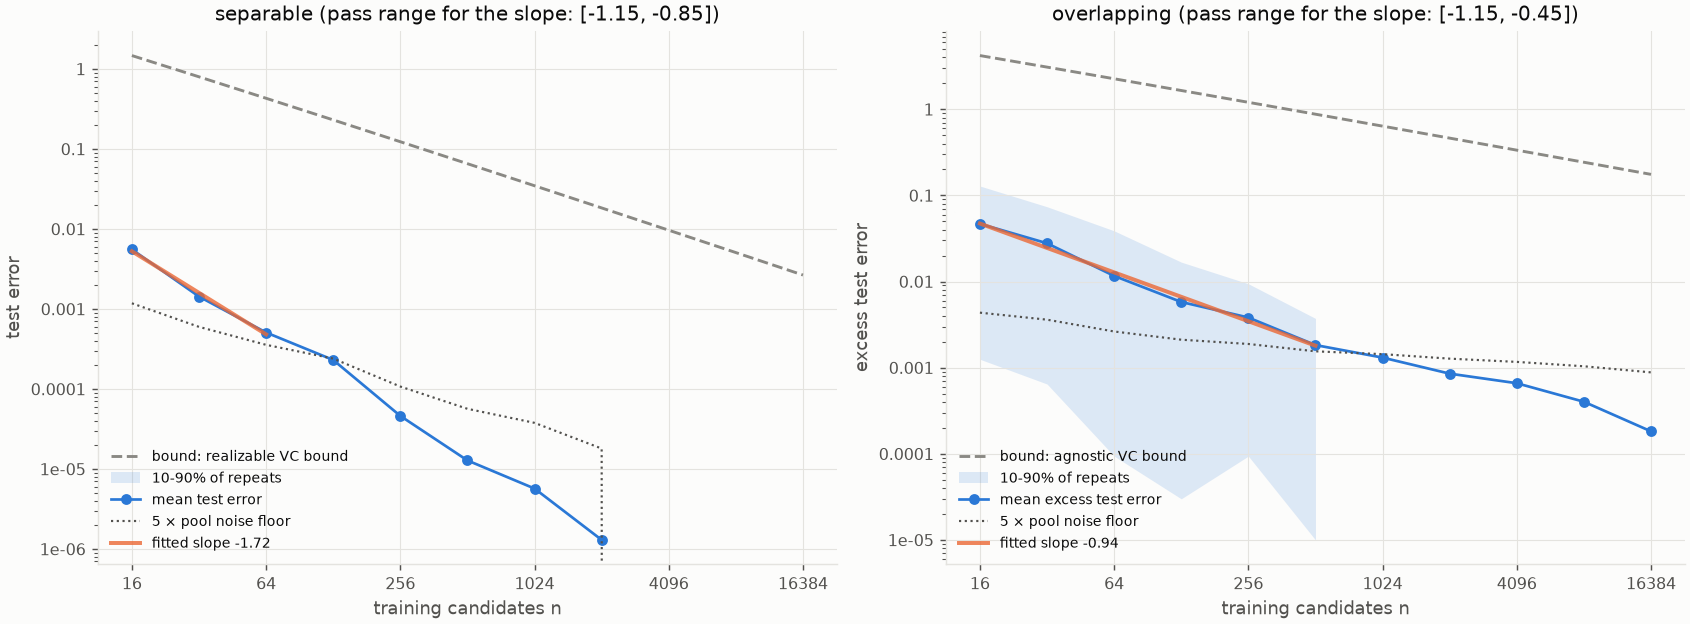
\includegraphics[width=0.8\linewidth]{../figures/e1_thresholds.png}
  \caption{E1: threshold ERM learning curves with the Result~1 bounds (dashed), the fitted slope
  and $5\times$ the pool noise floor. At $n=\EOneNLast$ the agnostic bound is
  $\EOneOvlBoundRatioLast\times$ the measured mean excess.}
  \label{fig:e1}
\end{figure}
